%%
%% This file uses the ACM Master Article Template (acmart).
%%
%% For submission and review, use \documentclass[manuscript,review]{acmart}.
%% For camera ready, switch to \documentclass[sigconf]{acmart}
%% (or whichever template style is required for your publication).
%%
\documentclass[manuscript,review]{acmart}

%% \BibTeX command to typeset BibTeX logo in the docs
\AtBeginDocument{%
  \providecommand\BibTeX{{%
    Bib\TeX}}}

%% Rights management information.
\setcopyright{rightsretained}
\copyrightyear{2026}
\acmYear{2026}
\acmDOI{XXXXXXX.XXXXXXX}

%% Conference information.
\acmConference[Conference acronym 'XX]{Make sure to enter the correct
  conference title from your rights confirmation email}{June 03--05,
  2018}{Woodstock, NY}
\acmISBN{978-1-4503-XXXX-X/2018/06}

%%
%% end of the preamble, start of the body of the document source.
\begin{document}

%%
%% The "title" command has an optional parameter,
%% allowing the author to define a "short title" to be used in page headers.
\title{Do LLM Personas Decide Like Real Users? A Study of Value-Choice Coherence Across Expertise Levels}

%%
%% Authors and affiliations.
%% All five authors share the same affiliation but each must be defined
%% separately for accurate metadata identification.
\author{Ritik Hariani}
\authornote{All authors contributed equally to this work.}
\email{ritikh2@illinois.edu}
\affiliation{%
  \institution{University of Illinois Urbana-Champaign}
  \city{Urbana-Champaign}
  \state{Illinois}
  \country{USA}
}

\author{Anil Muthigi}
\authornotemark[1]
\email{muthigi2@illinois.edu}
\affiliation{%
  \institution{University of Illinois Urbana-Champaign}
  \city{Urbana-Champaign}
  \state{Illinois}
  \country{USA}
}

\author{Saurav Nayak}
\authornotemark[1]
\email{sgnayak2@illinois.edu}
\affiliation{%
  \institution{University of Illinois Urbana-Champaign}
  \city{Urbana-Champaign}
  \state{Illinois}
  \country{USA}
}

\author{Jyoti Rawat}
\authornotemark[1]
\email{jrawat2@illinois.edu}
\affiliation{%
  \institution{University of Illinois Urbana-Champaign}
  \city{Urbana-Champaign}
  \state{Illinois}
  \country{USA}
}

\author{Rashi Tyagi}
\authornotemark[1]
\email{rtyagi4@illinois.edu}
\affiliation{%
  \institution{University of Illinois Urbana-Champaign}
  \city{Urbana-Champaign}
  \state{Illinois}
  \country{USA}
}

%%
%% A shorter author list for the page headers.
\renewcommand{\shortauthors}{Hariani, Muthigi, Nayak, Rawat, and Tyagi}

%%
%% The abstract is a short summary of the work to be presented in the
%% article.
\begin{abstract}
Persona-conditioned LLMs are increasingly used as stand-ins for human participants in HCI research, yet little work has tested whether they replicate the decision-making patterns that actually distinguish real users. We ran a controlled comparison of value-choice coherence between 14 LLM personas (Gemini 2.5 Flash-Lite, 7 expert and 7 novice photographers, 10 runs each) and 14 screened human participants on a multi-attribute camera-purchasing task. All participants ranked 11 camera attributes by personal priority, then selected between 15 camera pairs presented at three complexity levels (3, 6, or 11 visible attributes). We measured alignment between stated priorities and actual choices, how that alignment changed with complexity, and how closely LLM and human patterns matched. On aggregate the two populations appear similar (mean similarity score = 0.953), but the cross-condition Pearson correlation is near zero (\textit{r} = 0.066), and the patterns diverge in direction. Human expert alignment degrades as complexity increases; LLM expert alignment improves. The expert-novice gap reverses sign at the highest complexity level. LLM novice personas are a reasonable proxy for human novices; LLM expert personas are not. These findings show that high-level outcome metrics can mask fundamentally different decision processes, and suggest that evaluating LLM-based synthetic users requires condition-level, process-oriented comparisons rather than aggregate alignment scores.\footnote{Code, prompts, and data: \url{https://github.com/Saurav51/cs568-project}}
\end{abstract}

%%
%% CCS concepts and user-defined keywords.
\begin{CCSXML}
<ccs2012>
<concept>
<concept_id>10003120.10003121.10003122.10003334</concept_id>
<concept_desc>Human-centered computing~User studies</concept_desc>
<concept_significance>500</concept_significance>
</concept>
<concept>
<concept_id>10003120.10003121.10003122.10003333</concept_id>
<concept_desc>Human-centered computing~Empirical studies in HCI</concept_desc>
<concept_significance>300</concept_significance>
</concept>
<concept>
<concept_id>10010147.10010257.10010293</concept_id>
<concept_desc>Computing methodologies~Natural language processing</concept_desc>
<concept_significance>100</concept_significance>
</concept>
</ccs2012>
\end{CCSXML}

\ccsdesc[500]{Human-centered computing~User studies}
\ccsdesc[300]{Human-centered computing~Empirical studies in HCI}
\ccsdesc[100]{Computing methodologies~Natural language processing}

%%
%% Keywords. The author(s) should pick words that accurately describe
%% the work being presented. Separate the keywords with commas.
\keywords{LLM personas, decision-making, value-choice alignment, expertise, human-AI comparison}

%%
%% This command processes the author and affiliation and title
%% information and builds the first part of the formatted document.
\maketitle

\section{Introduction}
Large Language Models (LLMs) are increasingly used in HCI research to simulate human behavior across user feedback generation, usability evaluation, and early-stage design testing \cite{hamalainen2023synthetichci, park2023generativeagents}. Persona-conditioned LLMs---assigned demographics, expertise levels, or behavioral traits through prompting---promise cost-effective alternatives to human recruitment \cite{argyle2023out, aher2023usinglargelanguagemodels}. However, existing evaluations focus on whether outputs are plausible or useful rather than whether they reflect real human decision processes \cite{hamalainen2023synthetichci, salminen2025syntheticusers}. LLMs can produce surface-level human-like responses while failing on context-dependent behavior \cite{santurkar}, and persona grounding through prompting alone may not faithfully represent the cognitive characteristics the persona claims \cite{aher2023usinglargelanguagemodels, shanahans}.

Decision science has long established that human choices are shaped by task complexity, information availability, and expertise \cite{payne1993adaptive}. Experts apply domain knowledge consistently across contexts, whereas novices rely on surface-level cues as complexity increases \cite{payne1993adaptive}. Value-choice inconsistency---where stated preferences diverge from actual choices---is well-documented under cognitive load \cite{Tversky}. Whether persona-conditioned LLMs replicate these patterns across complexity levels is an open question.

We address this through a controlled comparison of value-choice coherence on a multi-attribute camera-purchasing task. We created 14 LLM personas using Gemini 2.5 Flash-Lite (7 experts, 7 novices) with detailed biographical backstories, and recruited 14 human participants screened to match the same expertise levels. All participants ranked 11 camera attributes by priority, then selected between camera pairs presented at three complexity levels: simple (3 attributes), moderate (6), and complex (11). We organize our study around two research questions evaluated through three metrics. \textbf{RQ1 (Expertise and Alignment)}: Do expert LLM personas demonstrate higher value-choice alignment than novice personas, and does this difference reflect the alignment gap observed between human experts and novices? \textbf{RQ2 (Complexity and Robustness)}: Does value-choice alignment decrease as product description complexity increases, and do expert personas exhibit greater robustness compared to novice personas? Our three metrics---\textbf{value-choice alignment} (whether choices match stated priorities), \textbf{consistency degradation} (whether alignment drops with complexity), and the \textbf{human-LLM persona gap}---evaluate whether LLM persona decision patterns match human counterparts.

Rather than evaluating synthetic users on output plausibility alone, we evaluate through decision-theoretic signals: multi-attribute reasoning, expertise effects, and value-choice consistency. We find that while aggregate metrics suggest closeness (similarity = 0.953), the cross-condition Pearson correlation is nearly zero ($r = 0.066$), and the direction of complexity effects diverges sharply. LLM expert personas \emph{improve} in alignment as complexity rises, inverting the degradation pattern observed in human experts. These results suggest surface-level proxies should not be treated as evidence of behavioral validity, motivating process-level evaluation of LLM-based user simulation.

\section{Related Work}
Simulation has long supported HCI design decisions \cite{murraysmith2022simulation}; LLMs extend this by generating synthetic user data. H\"am\"al\"ainen et al.\ show LLMs can produce realistic user content but raise ecological-validity concerns \cite{hamalainen2023synthetichci}, while SimUser simulates diverse personas for usability feedback at scale \cite{xiang2024simuser}. Generative agents demonstrate coherent interactive behaviors \cite{park2023generativeagents}, yet these approaches evaluate synthetic users by plausibility rather than decision processes; recent work shows LLM-simulated users can be unreliable proxies \cite{lostinsimulation2024, salminen2025syntheticusers}. Decision-making research shows human choices are shaped by complexity, information availability, and expertise \cite{payne1993adaptive}; experts apply domain knowledge consistently while novices use surface-level cues \cite{chi1988nature, shanteau1992competence}. Preference reversals demonstrate that stated and revealed preferences diverge under varying conditions \cite{slovic1983preference}. In human-AI interaction, decision outcomes depend on how users interpret model outputs \cite{bansal2021does}; LLMs approximate response patterns but fail on context-dependent behavior \cite{argyle2023out}. Our work bridges these areas by testing whether persona-conditioned LLMs exhibit human-like decision behavior rather than merely producing plausible outputs, using decision-theoretic concepts (multi-attribute reasoning, expertise effects, preference-choice consistency) to compare LLM personas with humans across expert/novice conditions and varied complexity.

\section{Methodology}

\subsection{LLM Personas}
We created 14 personas (7 experts, 7 novices) and ran each through Gemini 2.5 Flash-Lite. Expert personas span professional photography contexts (wedding/portrait, wildlife, street/documentary, commercial product, landscape/astrophotography, fashion editorial, sports); novice personas span casual contexts (college student, parent, food blogger, retired beginner, travel enthusiast, fitness-content creator, event planner). Rather than labeling personas ``expert'' or ``novice'' and telling them what to care about, we wrote each a detailed backstory covering gear, experience, knowledge, and purchase context (example prompts in Appendix~\ref{app:persona-prompts}), so priorities emerge naturally from context. We chose 14 personas over two archetypes because real users vary within groups: a sports photographer and a wedding photographer are both experts but trade off attributes differently. Prompts were fixed across runs. We ran each persona 10 times for 140 sessions total, using temperature 0.75, top-p 0.95, and 1024 max output tokens. Temperature was kept above zero so responses varied meaningfully across runs.

\subsection{Human Participants}
We recruited 14 participants (7 experts, 7 novices) over four weeks through outreach to two campus photography clubs and personal contacts. Recruitment was conducted by the authors; participation was voluntary and unpaid. Of 21 individuals approached, 14 met screening criteria; 7 were screened out for not meeting expert or novice definitions.

Screening was conducted in two passes. First, candidates answered qualifying questions verbally before being invited: experts had to (a) own at least three cameras, (b) report purchasing camera gear in the previous two years, and (c) explain at least two of \{aperture, ISO, shutter speed, RAW vs.\ JPEG\} in their own words. Novices had to (a) primarily use a phone for photography, (b) have never purchased a dedicated camera, and (c) self-identify as not familiar with manual camera controls. The same questions were repeated as self-report items on the Google Form to flag any verbal-vs.-recorded inconsistency (none were flagged). Participants completed the form anonymously (see Figure~\ref{fig:google-form} in Appendix~\ref{app:google-form}), following the same fixed order as LLM sessions (5 simple $\rightarrow$ 5 moderate $\rightarrow$ 5 complex). Informed consent was obtained; identifying information was not collected.

\subsection{Stimuli}
We worked with 11 camera attributes: price, image quality, battery life, optical zoom, weight, ease of use, manual controls, RAW support, burst speed, weather sealing, and 4K video. Camera names and specs were generated synthetically using Claude; names were fictional (e.g., ``Alvex T1,'' ``Brikon S2'') to avoid brand-recognition bias, and attribute values were set so each pair had no obvious winner. Complexity was defined by the number of visible attributes per pair: 3 (simple), 6 (moderate), or all 11 (complex). Five pairs per complexity level (15 total) used different attribute subsets within each level so no single trade-off dominated. Table~\ref{tab:camera-pair} shows an example simple-condition pair.

\begin{table}[h]
  \caption{Example simple-condition camera pair (3 visible attributes). Each camera has a clear strength: Alvex T1 wins on price and battery, Brikon S2 wins on image quality. There is no dominant option; the participant's choice depends on which attribute they ranked highest in the priority-elicitation step.}
  \label{tab:camera-pair}
  \centering
  \begin{tabular}{l r r}
    \toprule
    \textbf{Attribute} & \textbf{Alvex T1} & \textbf{Brikon S2} \\
    \midrule
    Price          & \$289   & \$499   \\
    Image quality  & 6/10    & 9/10    \\
    Battery life   & 18 hrs  & 11 hrs  \\
    \bottomrule
  \end{tabular}
\end{table}

\subsection{Session Structure}
Each session covered all 15 pairs. For LLM personas this was a multi-turn conversation; for humans, the same structure via Google Form. \textbf{Persona setup} (LLM only): the biographical prompt was loaded at session start and kept constant. \textbf{Priority ranking}: before seeing any cameras, participants ranked all 11 attributes by importance. Eliciting priorities first locks in the stated preference choices are scored against; reversing the order would let participants rationalize the ranking from their choices, making the comparison circular. \textbf{Camera pairs}: presented one at a time in fixed order (5 simple, 5 moderate, 5 complex). Only attributes in the pair's subset were shown in plain language. Participants picked a camera and reported the decisive attribute (\texttt{Choice: [camera name]}, \texttt{Decisive attribute: [attribute name]}); the decisive attribute was collected for future process-level analysis but is not used in the metrics here. Fixed order ensures any carryover effects apply equally across participants.

\subsection{Evaluation Metrics}
\textbf{Value Choice Alignment.} For each pair, let $D$ be the set of visible attributes on which the two cameras differ, with $n = |D|$. We sort $D$ by the participant's Turn-1 priority ranking and assign linear weights $w_k = n - k + 1$ to the attribute at rank $k$. Let $c_k = 1$ if the chosen camera is objectively better on attribute $k$ (per the directionality in \texttt{attributes.json}, e.g., lower price is better) and $c_k = 0$ otherwise. The pair score is
\begin{equation}
\mathrm{VCA}_{\text{pair}} = \frac{\sum_{k=1}^{n} w_k \, c_k}{\sum_{k=1}^{n} w_k}.
\end{equation}
For a session $s$ at complexity $\ell$ (five pairs $P_{s,\ell}$), $\mathrm{VCA}_{s,\ell} = \frac{1}{5}\sum_{p \in P_{s,\ell}} \mathrm{VCA}_{\text{pair}}(p)$. For LLM personas, persona-level scores are the mean of 10 runs; group scores aggregate across the 7 personas per label $L \in \{\text{expert}, \text{novice}\}$. All aggregates lie in $[0,1]$, where 1 indicates perfect alignment and 0 indicates every choice contradicted the stated ranking. We use a graded $[0,1]$ score rather than a binary top-attribute hit rate so partial alignment is captured: a choice that satisfies the 2nd- and 3rd-ranked priorities but not the 1st is meaningfully different from one satisfying none, and the $[0,1]$ scale preserves that distinction.

\textbf{Consistency Degradation.} Rather than fitting a regression, we measured alignment change at two transitions: simple $\rightarrow$ moderate and moderate $\rightarrow$ complex. For a session $s$:
\begin{equation}
\Delta_{s,\,\ell_1 \rightarrow \ell_2} = \mathrm{VCA}_{s,\ell_2} - \mathrm{VCA}_{s,\ell_1}.
\end{equation}
Negative $\Delta$ indicates degradation; positive indicates improvement. Differences were averaged across 10 runs per persona, then 7 personas per group.

\textbf{Human-LLM Persona Gap.} For each of the six (label $\times$ complexity) cells, let $\mathrm{VCA}^{\text{LLM}}_{L,\ell}$ and $\mathrm{VCA}^{\text{H}}_{L,\ell}$ denote LLM and human group means; the signed gap is $g_{L,\ell} = \mathrm{VCA}^{\text{LLM}}_{L,\ell} - \mathrm{VCA}^{\text{H}}_{L,\ell}$. We compute a similarity score
\begin{equation}
S = 1 - \frac{1}{6}\sum_{L,\ell} |g_{L,\ell}|,
\end{equation}
lying in $[0,1]$ (1 = exact match), and a Pearson correlation between LLM and human scores across the six cells. Similarity captures whether populations land in the same numerical range; correlation captures whether they respond to expertise and complexity in the same direction. These can disagree sharply (Section~\ref{sec:results}). All analysis is descriptive; no inferential model was fit.

\section{Results}\label{sec:results}
We report results across three metrics: value-choice alignment (VCA), consistency degradation, and the human-LLM persona gap.

\subsection{Value-Choice Alignment}
Figure~\ref{fig:vca-plot} and Table~\ref{tab:gap} (LLM and Human columns) summarize mean VCA scores. LLM experts score 0.506, 0.558, 0.605 (simple/moderate/complex); LLM novices 0.657, 0.541, 0.558. Humans score 0.590, 0.527, 0.518 (experts) and 0.590, 0.535, 0.549 (novices). Across complexity, LLMs average 0.556 (expert) and 0.585 (novice); humans 0.545 and 0.558. The LLM-expert curve rises while every other curve declines or stays flat.

\begin{figure}[h]
  \centering
  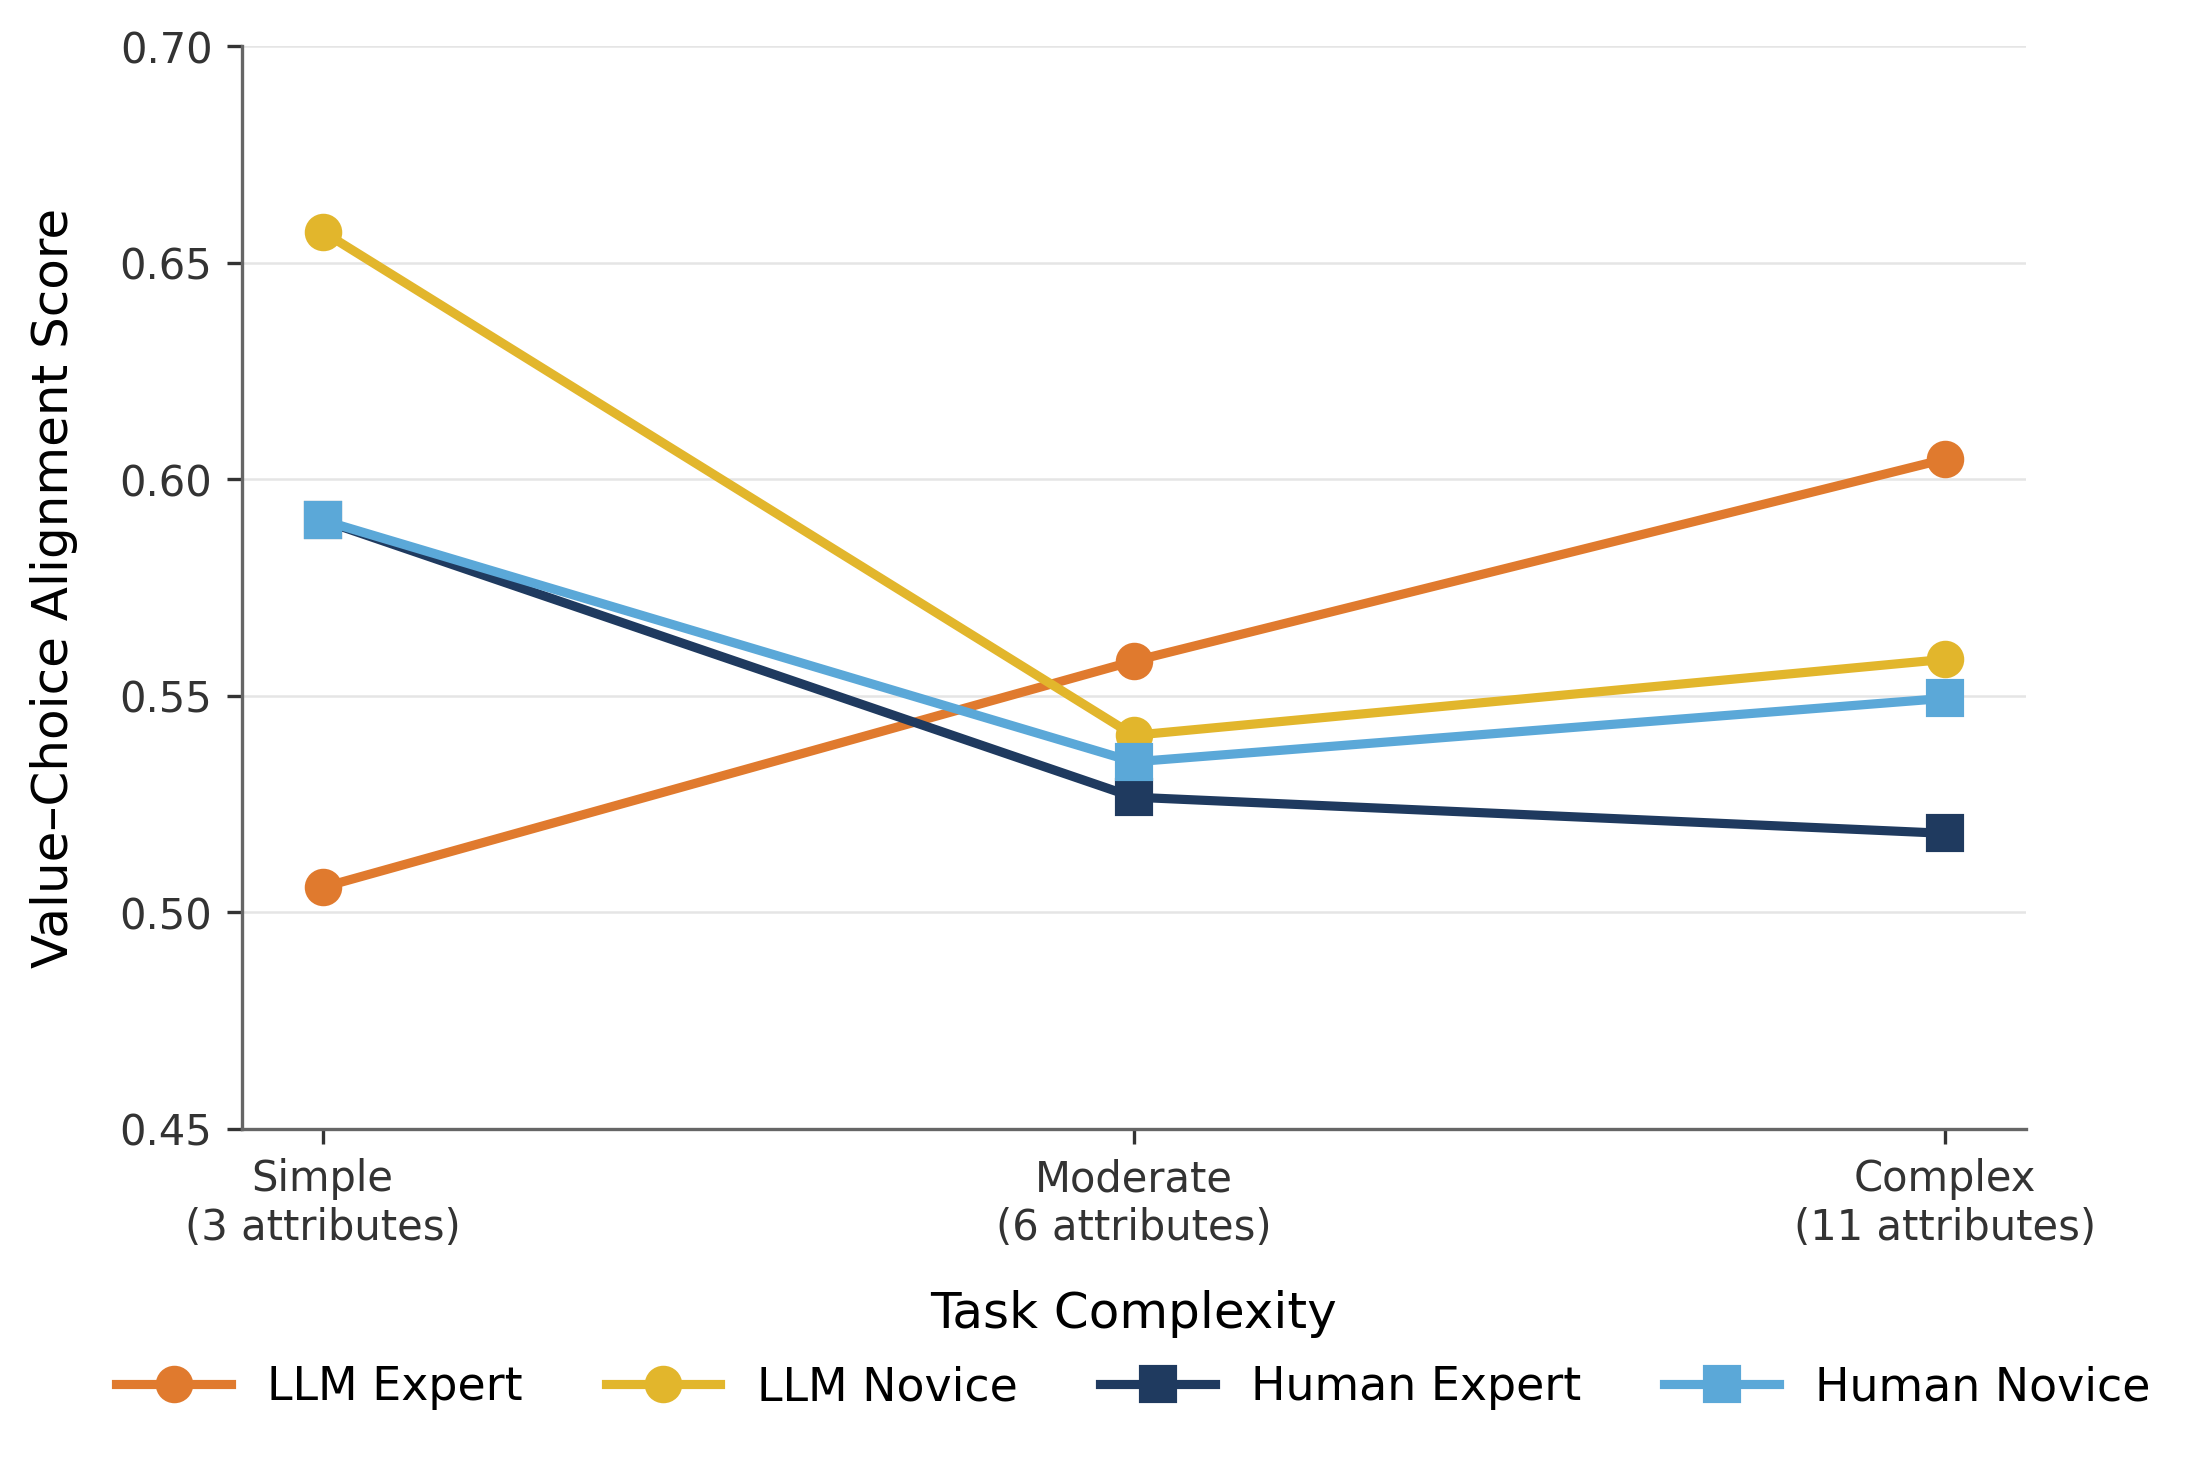
\includegraphics[width=0.45\linewidth]{vca-by-complexity.png}
  \caption{Mean value-choice alignment across complexity levels (1 = simple, 2 = moderate, 3 = complex) for the four groups. Human experts and novices both decline as more attributes are introduced, consistent with the well-documented degradation of value-choice coherence under cognitive load. LLM experts move in the opposite direction --- alignment \emph{rises} from simple to complex --- and the expert-novice ordering crosses between simple and complex, in a way that humans never do.}
  \Description{Line plot showing mean value-choice alignment on the y-axis against complexity level on the x-axis for four groups: human experts, human novices, LLM experts, and LLM novices. Human expert and human novice curves both decline as complexity increases. The LLM novice curve drops sharply from simple to moderate then stabilizes. The LLM expert curve rises monotonically from simple to complex, crossing the LLM novice curve between the simple and complex conditions.}
  \label{fig:vca-plot}
\end{figure}

\subsection{Consistency Degradation}
Human experts drop at both transitions (simple $\rightarrow$ moderate $= -0.064$; moderate $\rightarrow$ complex $= -0.008$). Human novices drop then slightly recover ($-0.056$, $+0.015$). LLM experts \emph{improve} at both ($+0.052$, $+0.047$). LLM novices drop sharply then stabilize ($-0.116$, $+0.018$).

\subsection{Human-LLM Persona Gap}
Across the six (label $\times$ complexity) conditions, the mean absolute gap is 0.047 and the mean signed gap is $+0.019$, yielding a similarity score of 0.953. The Pearson correlation between LLM and human scores across the six conditions is 0.066---effectively zero. Table~\ref{tab:gap} reports the per-condition breakdown. Largest gaps fall on expert/simple ($-0.085$) and expert/complex ($+0.086$); smallest on novice/moderate ($+0.006$) and novice/complex ($+0.009$). The expert-novice gap within each population diverges by complexity: at simple, LLM novices outscore LLM experts by 0.151 while humans are tied; at complex, LLM experts outscore LLM novices by 0.046 while human experts score 0.031 \emph{below} novices---a sign reversal.

\begin{table}[h]
  \caption{Per-condition signed gap (LLM minus human). Bold entries mark the two largest absolute gaps (both in the expert subgroup); italic entries mark the two near-zero gaps (both in the novice subgroup). The pattern --- large expert gaps with opposite signs, near-zero novice gaps --- is what produces a high aggregate similarity (0.953) alongside a near-zero pooled Pearson correlation ($r = 0.066$).}
  \label{tab:gap}
  \centering
  \begin{tabular}{l l r r r}
    \toprule
    \textbf{Label} & \textbf{Complexity} & \textbf{LLM} & \textbf{Human} & \textbf{Gap} \\
    \midrule
    Expert & Simple   & 0.506 & 0.590 & \textbf{$-0.085$} \\
    Expert & Moderate & 0.558 & 0.527 & $+0.031$ \\
    Expert & Complex  & 0.605 & 0.518 & \textbf{$+0.086$} \\
    Novice & Simple   & 0.657 & 0.590 & $+0.067$ \\
    Novice & Moderate & 0.541 & 0.535 & \emph{$+0.006$} \\
    Novice & Complex  & 0.558 & 0.549 & \emph{$+0.009$} \\
    \bottomrule
  \end{tabular}
\end{table}

\subsection{Label-Stratified Correlation}
The pooled $r = 0.066$ above hides label-specific patterns. Computing the Pearson correlation separately within each label is more diagnostic: across the three complexity levels, the within-novice correlation is $r_{\text{novice}} = +0.993$ and the within-expert correlation is $r_{\text{expert}} = -0.927$ ($n=3$ per label). LLM novice scores rise and fall with human novices almost perfectly; LLM expert scores move opposite to humans at nearly the same magnitude. These near-equal-and-opposite effects cancel when pooled, collapsing the aggregate correlation despite a near-perfect within-novice fit and strongly inverted within-expert fit. Both values are computed on three points and should be read as direction-of-effect indicators.

\textbf{Key Findings.} The high similarity (0.953) and small mean absolute gap (0.047) suggest LLM and human scores are numerically close, but the near-zero pooled correlation reveals they do not track the same pattern. Stratifying makes this explicit: within novices, scores rise and fall together ($r=+0.993$); within experts, they move in opposite directions ($r=-0.927$); the two cancel when pooled. The disagreement concentrates in the expert subgroup. \textbf{LLM experts invert the human complexity trend}: humans score highest at simple (0.590) and lowest at complex (0.518); LLM experts do the opposite (0.506 $\rightarrow$ 0.605). \textbf{The expert-novice gap reverses direction at complex}: humans show novices ahead by 0.031; LLMs show experts ahead by 0.046. \textbf{LLM novice personas are a reasonable proxy for human novices} (negligible gaps at moderate, $+0.006$, and complex, $+0.009$); \textbf{LLM expert personas are not}---the largest single mismatch is expert/simple ($-0.085$), where humans are tied at 0.590 but LLM novices (0.657) massively outscore LLM experts (0.506). A single-number similarity score would have falsely characterized these populations as well aligned; the condition-level breakdown and cross-condition correlation show this agreement is largely coincidental, motivating process-level evaluation.

\section{Conclusion}
Our two research questions converge on the same conclusion across all three metrics.

On \textbf{RQ1 (Expertise and Alignment)}, expert LLM personas do not show higher value-choice alignment than novices; they score lower on average (0.556 vs.\ 0.585). More critically, this gap does not reflect the human pattern. Human experts and novices are tied at simple (0.590 each), and human novices slightly outperform experts at complex (gap $= -0.031$). LLMs show the inverse: at simple, novices massively outscore experts (0.657 vs.\ 0.506); at complex, experts lead (0.605 vs.\ 0.558, gap $= +0.046$). Labeling a persona ``expert'' through prompting does not produce expert-like decision-making. The failure is asymmetric: LLM novices are reasonable proxies for human novices, particularly at moderate and complex (gaps $+0.006$, $+0.009$); LLM experts are not.

On \textbf{RQ2 (Complexity and Robustness)}, the populations diverge in opposite directions. Human experts show expected degradation ($-0.064$, $-0.008$); LLM experts invert it, improving at both transitions ($+0.052$, $+0.047$). LLM experts do not exhibit greater robustness in any human-like sense---they exhibit a fundamentally different response. LLM novices degrade sharply then stabilize ($-0.116$, $+0.018$), at least matching the direction of human novice degradation ($-0.056$) if not magnitude.

The Human-LLM Gap shows why this matters. Aggregate scores look fine: similarity 0.953, mean absolute gap 0.047. But the cross-condition Pearson correlation is near zero ($r = 0.066$), meaning the populations land in the same range by coincidence, not because they respond to expertise and complexity the same way. The largest gaps fall exactly where expert behavior diverges most, at simple ($-0.085$) and complex ($+0.086$). We call this the \emph{single-number trap}: any one-shot summary---similarity score, mean absolute gap, overall accuracy---can be high while underlying decision processes are completely different. A reviewer seeing only 0.953 would conclude these LLM personas are a strong proxy; the 0.066 correlation, inverted complexity trend, and sign reversal at complex say the opposite.

These findings suggest that persona prompting does not ground ``expertise'' in a way that produces human-like decision behavior, and that aggregate metrics obscure this. For HCI work using LLM-based synthetic users, outcome-level proxies should not be treated as behavioral validity; researchers must evaluate whether synthetic users replicate the \emph{patterns} of degradation, expertise, and trade-off that motivate the simulation. Process-level validation, scaled across model families and domains, is the demanding bar this work points toward. Detailed limitations of the present study and concrete future-work directions are provided in Appendices~\ref{app:limitations} and~\ref{app:future}.

%%
%% The acknowledgments section is defined using the "acks" environment
%% (and NOT an unnumbered section). This ensures the proper
%% identification of the section in the article metadata, and the
%% consistent spelling of the heading.
% \begin{acks}
% Acknowledgments go here.
% \end{acks}

%%
%% The next two lines define the bibliography style to be used, and
%% the bibliography file.
\bibliographystyle{ACM-Reference-Format}
\bibliography{sample}

%%
%% Appendix.
\appendix

\section{Google Form Used by Human Participants}\label{app:google-form}

\begin{figure*}[h]
  \centering
  \includegraphics[width=\textwidth]{google-form-screenshots.png}
  \caption{The Google Form used by human participants. Left: the screening item and the priority-ranking matrix over all 11 attributes. Right: example camera-pair items (one simple, one complex) showing only the attributes belonging to that pair. The form mirrors the LLM session structure: ranking first, then 15 pairs in the fixed simple~$\rightarrow$~moderate~$\rightarrow$~complex order.}
  \Description{Composite screenshot of the Google Form used by human participants. The left panel shows the expertise screening item followed by a matrix in which respondents rank all eleven camera attributes from most to least important. The right panel shows two example camera-pair items: a simple pair with three visible attributes and a complex pair with all eleven visible attributes. Each pair lists the two camera names, their attribute values, and the response fields for choice and decisive attribute.}
  \label{fig:google-form}
\end{figure*}

\section{Example Persona System Prompts}\label{app:persona-prompts}

\begin{table*}[h]
  \caption{Two example persona system prompts shown side by side: one expert and one novice. Backstories specify gear, experience, and purchase context, but never instruct the persona on which attributes to prioritize. The remaining 12 prompts (6 expert, 6 novice) follow the same structure across other photography contexts.}
  \label{tab:persona-prompts}
  \centering
  \footnotesize
  \begin{tabular}{p{0.46\textwidth} p{0.46\textwidth}}
    \toprule
    \textbf{Expert (EXP\_01) --- Marcus Chen} & \textbf{Novice (NOV\_01) --- Aisha Williams} \\
    \midrule
    You are Marcus Chen, a 38-year-old professional wedding and portrait photographer based in Chicago. You have been shooting professionally for 12 years and run your own photography business, handling weddings on weekends, engagement sessions during the week, and occasional editorial or studio portrait work.
    &
    You are Aisha Williams, a 21-year-old college student who takes all her photos on her iPhone 15 Pro. You have never owned a dedicated camera, and your photography knowledge comes from social media, TikTok tutorials, and trial and error on your phone. \\
    \addlinespace
    You own 6 cameras, including a Sony A7R V, a Canon R5, and several Fujifilm bodies. Over the last two years you have spent more than \$40{,}000 on cameras, lenses, lighting equipment, and accessories. You shoot RAW exclusively and edit your images in Lightroom and Capture One.
    &
    You edit photos in apps like VSCO and Lightroom Mobile and post to Instagram. You are familiar with features like portrait mode, night mode, and filters from using your phone camera regularly, and you take photos mostly in casual day-to-day situations --- around campus, with friends, and on trips. \\
    \addlinespace
    You understand aperture, ISO, shutter speed, dynamic range, color science, lens rendering, autofocus tracking, and post-processing workflows. You have shot in dim reception halls, bright outdoor ceremonies, churches lit only by candles, and controlled studio environments.
    &
    You have heard terms like aperture, ISO, and shutter speed but you don't really know what they mean. Photography interests you as a hobby, and you have recently started wondering whether a dedicated camera would let you take photos you can't easily capture with your phone. \\
    \bottomrule
  \end{tabular}
\end{table*}

\section{Limitations}\label{app:limitations}

Our human sample is small ($N = 14$; 7 experts, 7 novices), recruited through convenience sampling without compensation, limiting statistical power and biasing toward photography enthusiasts. All LLM data come from a single model (Gemini 2.5 Flash-Lite) under one prompting configuration; behavior may differ across model families or sizes, so our results should not be read as a general claim about LLM personas. Camera stimuli were generated by a different LLM (Claude), avoiding hand-curated experimenter bias but introducing potential distributional alignment with one model family. The domain is low-stakes consumer choice; whether the inverted complexity trend in LLM experts generalizes to higher-stakes domains (medical, financial, legal) is an open question. We report only descriptive statistics; the directional effects highlighted (particularly the inverted complexity trend and sign reversal of the expert-novice gap at complex) should therefore be treated as suggestive rather than confirmatory, and the cross-condition correlations are computed on small $n$ (6 cells overall, 3 per label) and should be read as direction-of-effect indicators rather than precise estimates. Finally, the priority ranking was single-shot without practice rounds, and pair order was fixed (simple $\rightarrow$ moderate $\rightarrow$ complex) for both populations, bundling session-internal learning and fatigue into the complexity manipulation.

\section{Future Work}\label{app:future}

Four directions follow. First, the divergent complexity trends in RQ2 are descriptive; the natural confirmatory test is a mixed-effects logistic regression with persona label, complexity, and their interaction as fixed effects and persona nested within label as a random effect, which requires enlarging the human sample. Second, replicating the protocol across model families (GPT-class, Claude-class, open-weight models) and sizes will determine whether value-choice degradation under complexity, and its inversion in LLM experts, is a property of one model or a general property of persona-conditioned LLMs. Third---and we view this as most important---the contrast between high aggregate similarity (0.953) and near-zero per-condition correlation ($r = 0.066$) is itself a methodological finding: HCI evaluation of LLM-based synthetic users needs metrics that capture decision \emph{processes} (which attributes drive each choice, how priority is traded against attribute values, where the model deviates from its own stated ranking) rather than only outcome-level alignment. Fourth, extending to higher-stakes domains will test whether the LLM-expert-improving-with-complexity pattern is general or an artifact of low-stakes consumer choice. A more speculative direction addresses RQ1 directly: whether richer expertise grounding (retrieval over domain knowledge, few-shot expert traces, or chain-of-thought elicitation) can close the LLM-human expert gap.

\end{document}
